\documentclass[conference]{IEEEtran}

% Language setting
% Replace `english' with e.g. `spanish' to change the document language
\usepackage[english]{babel}

% Set page size and margins
% Replace `letterpaper' with `a4paper' for UK/EU standard size
\usepackage[letterpaper,top=2cm,bottom=2cm,left=3cm,right=3cm,marginparwidth=1.75cm]{geometry}

% Useful packages
\usepackage{amsmath}
\usepackage{graphicx}
\graphicspath{ {./images/} }

\usepackage[colorlinks=true, allcolors=blue]{hyperref}

\title{Virtual Personal Assistant (VPA) for Bengali with Machine Learning (ML) and Reinforcement Learning (RL)}
%\author{Sadidul Islam}
\author{\IEEEauthorblockN{Sadidul Islam}
\IEEEauthorblockA{\textit{Student, MSCSE} \\
\textit{United Internation University}\\
Bangladesh \\
sadid@soceton.com}
%\and
%\IEEEauthorblockN{2\textsuperscript{nd} Given Name Surname}
%\IEEEauthorblockA{\textit{dept. name of organization (of Aff.)} \\
%\textit{name of organization (of Aff.)}\\
%City, Country \\
%email address or ORCID}
}
\date{\today}

\begin{document}
\maketitle

\begin{abstract}
    In the current technological world, virtual personal assistants (VPA) have become necessary companions, offering seamless voice-activated interaction with technologies, personalized assistance, and streamlined task management for enhanced productivity and convenience.
    In this paper, propose a virtual personal assistant development with speech to text, chatbot functionality, and text to speech synthesis where speech to text is implemented as Reinforcement Learning model so that it can personalize the user specific voice characteristics.
    By leveraging chatbot capabilities, the assistant can engage in natural language conversations, understand user intents, and provide relevant responses.
    The text-to-speech synthesis component ensures that the VPA can generate human-like speech output, enhancing the user experience.
    The developed VPA showcases the potential of combining multiple technologies to create a versatile and user-friendly virtual assistant.
\end{abstract}

\section{Introduction}\label{sec:introduction}
Technology has made remarkable strides in recent years, revolutionizing the way we live, work, and connect with each other.
We can make life easier by having a personal assistant installed on a personal computer or mobile phone.
All the technologies require human interaction to operate, e.g.\ computer, mobile, IoT devices, etc.
There are situations that human can't provide proper interactions due to disabilities, lack of knowledge, and also for limited time as well.
A virtual personal assistant (VPA) is built with Machine Learning technologies such as Natural Language Processing (NLP), Speech Recognition, which can help in these situations by taking a voice command from the human and completing the tasks automatically.
For example, A virtual personal assistant (VPA) can be used to set a reminder, sending email, know weather information, search information in Google, update to-do list etc \cite{adheetee}.

Numerous works for the Virtual Personal Assistant (VPA) have been done for the English language throughout recent years.
Such as, Apple’s Siri \cite{siri}, Google’s Voice Actions \cite{google-mobile} and Google Now \cite{google-now}, Microsoft’s Bing Voice Search \cite{microsoft-tellme}, and Nuance’s Dragon Go! \cite{nuance-dragon} and Nina \cite{nuance-nina}, and many startup efforts like Speaktoit \cite{speaktoit}, and many more.

Bangla is the 7th most widely spoken language in the world, 272.7 million people around the world speak in Bangla \cite{mostspoken}.
Euromonitor International reports only 18\% of the total population in Bangladesh can understand and speak English \cite{english-speaker-bangladesh}.
In addition to that 25.34\% (literacy rate 74.66\% according to the Population and Housing Census 2022) of the total population is illiterate who cannot even read or write Bangla language \cite{litaracy-bangladesh}
According to Unicef Bangladesh 2.8 percent of the population and 1.7 per cent of children has at least one disability \cite{disabled-stats} in the country where Bengali is the primary language.
Among the disabled people 11.43 (0.32 percent in whole population) percent have limitations in speaking and other 88.57 percent can at least speak, but still they are away from technologies by other disabilities.

Although, very little work related to virtual personal assistant (VPA) had been done yet \cite{adheetee}.
We can't find any production grade virtual personal assistant (VPA) in Bengali language as of today.

In this research we propose a system with Speech to Text, Chatbot, and Text to Speech combined to develop a virtual personal assistant (VPA) that can help disabled (verbal) people to interact with technologies, save time for busy people by doing their technological tasks in no time wasted with just a voice command.
This virtual personal assistant will take voice commands and based on that voice command it will do some actions like calling someone, interact with IoT devices, etc.\ and reply with the required information to answer the users' voice command.
In other virtual personal assistant (VPA) we found that it lacks of personalizing for a specific person, but solution for this problem is more required when we consider a disabled person.
Because they might not speak properly like other people, if we don't consider this problem then it won't help them at all.
So, we introduce Reinforcement Learning (RL) for Speech to Text model to personalize user specific voice characteristics.
%Researching personal assistants with reinforcement learning offers several compelling reasons.
%Firstly, reinforcement learning allows personal assistants to learn from user interactions and improve over time.
%This enables them to provide more personalized and effective assistance, tailoring responses to individual preferences and needs.
%Secondly, reinforcement learning empowers personal assistants to make autonomous decisions, enabling them to
%handle complex tasks and adapt to changing circumstances.
%This flexibility enhances their ability to assist users in various contexts.
%Moreover, reinforcement learning can help personal assistants optimize their performance by continuously learning and refining their strategies.
%This research can revolutionize the field, creating smarter, more capable personal assistants that offer enhanced user experiences.

%We have reviewed several papers that are related to our problem to some extent.
%We have seen how to develop a self-improving chatbot based on reinforcement learning \cite{rl-chatbot}, also we have seen information about developing to deploying about Siri Experience \cite{siri-experience}.
%Both of the paper has mentioned a different kind of information about building a solution for building a personal assistant.
%They are solving similar problems in different ways and in small or broader ways.
%By combining the experience of these papers we can build a new solution of our own to make a better solution in this area.
%The purpose of this work is to create a universal personal assistant that can understand human voice/texts and decide as it was set up before.
%We have a lot of chatbots or even personal Assistants like Siri \cite{siri}, Google’s Voice Actions \cite{google-mobile}, and many more.
%These are more of a chatbot, and you can do very basic actions with them like open an app, search for something on the web or in any app, etc.
%Our assistant will take a decision based on previously provided rules based on a given scenario.
%For example, if someone wants to have an appointment with me, if it is once configured to set an appointment then it would set it or discuss with me and the person to set a suitable time and date.
%So, this solution is not just a chatbot, it would be what we call an assistant.


\section{Review}\label{sec:review}
%We have studied some papers for making a solution to our problem by combining them all possible papers.
%In the paper “Self-improving Chatbots based on Reinforcement Learning” \cite{rl-chatbot} we have found how to create a self-improving question and answering system.
%They have used Deep Q-Network (DQN) agent as the policy learning system with epsilon greedy exploration.
%It is implemented in a way that it can answer out-of-scope questions with a fallback answering system.
%If the answer is matched with 30\% or above confidence level then the NLU engine returns the response with the confidence, otherwise, it returns a fallback answer.
%The authors propose a setup where the chatbot acts as an RL agent, observing the state of the conversation, taking actions, and receiving rewards or penalties based on user satisfaction.
%The dialogue policy is learned by maximizing the expected cumulative reward over time.
%Designing suitable reward functions is crucial for effective RL. The paper suggests using user satisfaction as the reward signal, which can be derived from explicit ratings or implicit feedback.
%The authors discuss various reward-shaping techniques to enhance the learning process and encourage desirable behavior in the chatbot.
%
%
%In the paper titled "Large-Scale Personal Assistant Technology Deployment: The Siri Experience" \cite{siri-experience} we have found some of the very essential information about developing a personal assistant, the challenges they have faced, and how they have overcome them.
%In recent years, smartphones and other mobile devices, such as electronic tablets and more generally a wide variety of hand-held media appliances, have brought about an unprecedented level of ubiquity in computing and communications.
%At the same time, voice-driven human-computer interaction has benefited from steady improvements in the underlying speech technologies (largely from a greater quantity of labeled speech data leading to better models), as well as the relative decrease in the cost of computing power necessary to implement comparatively more sophisticated solutions.
%This has sparked interest in a more pervasive spoken language interface, in its most inclusive definition encompassing speech recognition, speech synthesis, natural language understanding, and dialog management.
%Multiple voice-driven initiatives have now reached commercial deployment, among others Apple’s Siri \cite{siri}, Google’s Voice Actions \cite{google-mobile} and Google Now \cite{google-now}, Microsoft’s Bing Voice Search \cite{microsoft-tellme}, and Nuance’s Dragon Go! \cite{nuance-dragon} and Nina \cite{nuance-nina}, and many startup efforts like Speaktoit \cite{speaktoit}.
%The well-publicized release of Siri in Apple’s iPhone 4S, in particular, may have heralded an irreversible shift toward the “intelligent personal assistant” paradigm: just say what you want, and the system will automatically figure out what the best course of action is.
Virtual personal assistant (VPA) has been researched and utilized by researchers over the decades.
In our literature work, we focused on latest works including research, production related information which are published on reliable sources.
Like, IEEE Digital Library, ACM Digital Library, Springer etc.
We have found a couple of research directly related to our works and there are some partially related works.
We have separated discussion of the researches in separate sections.

\subsection{Virtual Personal Assistant}\label{subsec:virtual-personal-assistant}
Adheetee: A Comprehensive Bangla Virtual Assistant is developed based on Natural Language Understanding (NLU) using Deep Learning (DL) models such as Recurrent Neural Network (RNN) for Bangla Language \cite{adheetee}.
They have collect and created their own corpus then trained the model on that dataset.

In the paper "Large-Scale Personal Assistant Technology Deployment, specifically in the context of the Siri Experience" \cite{siri-experience}, the researchers provided a lot of information about development and deployment a production grade Siri, Siri is a virtual personal assistant developed by Apple.
They have showed how they have implemented architecture, deployment architecture and how they have improved performance Natural Language Processing (NLP) and Natural Language Understanding (NLU) capabilities.

\subsection{Speech Recognition}\label{subsec:speech-recognition}
The paper State of Art Research in Bengali Speech Recognition \cite{speech-recog-bengali} presents a comprehensive methodology for advancing the field of Bengali speech recognition.
They have pointed out about challenges specific to Bengali speech recognition.
The researchers proposed a hybrid approach of that combines acoustic modeling, language modeling, and lexical modeling using Convolutional Neural Network (CNN), Recurrent Neural Network (RNN) to improve accuracy and performances.

\subsection{Chatbot}\label{subsec:chatbot}
The paper "Doly: Bengali Chatbot for Bengali Education" \cite{doly} presents the methodology employed to develop an intelligent chatbot named Doly, designed specifically for Bengali language education.
The methodology emphasizes the importance of continually updating and expanding Doly's knowledge base to keep up with evolving educational content and trends.

In the paper “Self-improving Chatbots based on Reinforcement Learning” \cite{rl-chatbot} we have found how to create a self-improving question and answering system.
They have used Deep Q-Network (DQN) agent as the policy learning system with epsilon greedy exploration.
The authors propose a setup where the chatbot acts as an RL agent, observing the state of the conversation, taking actions, and receiving rewards or penalties based on user satisfaction.


\section{Methodology}\label{sec:methodology}
Our solution has three machine learning (ML) components, Speech to Text, Chatbot, and Text to Speech.
Representing sounds or human voice in digital media involves converting them into analog signals.
The main challenge lies in converting these analog signals into text format, which enables machines to process and work with the data effectively, and the Speech to Text solves this problem\cite{speech-recog-bengali}.
A Chatbot is a computer program or an artificial intelligence which conducts a conversation via auditory or textual methods\cite{chatbot}.
Text-to-Speech (TTS) is a technology that converts written text into spoken words\cite{text-to-speech}.

\begin{figure}
    \centering
    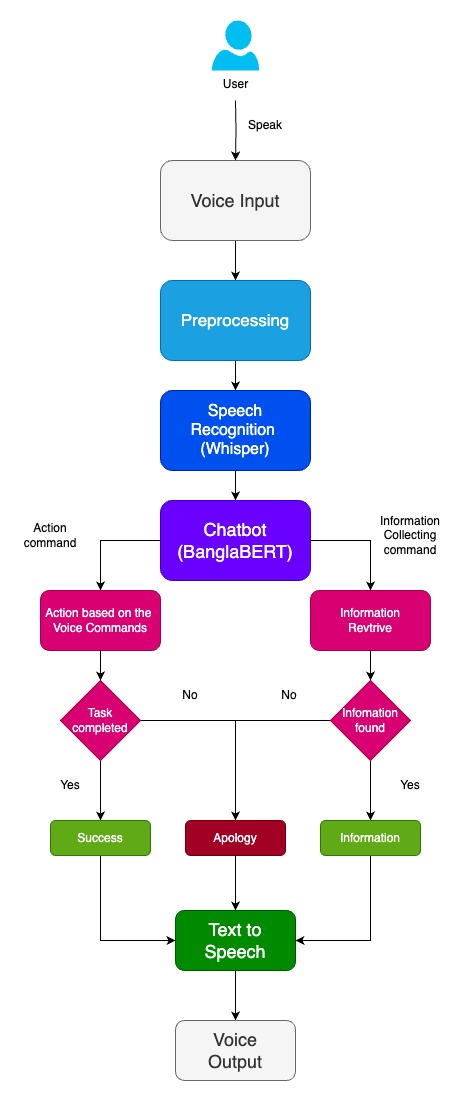
\includegraphics[width=0.4\textwidth]{Methodology-diagram}
    \caption{Flowchart of the system}\label{fig:methodology}
\end{figure}

Figure \ref{fig:methodology} shows a user provides a voice input, then our system processes the voice data and provides text data from Speech-to-Text (BanglaSTT)\cite{bangla-stt} model.
Speech to Text returns text data for the voice data, this data is the input of the chatbot (BanglaBERT)\cite{bangla-bert}, chatbot takes the decision, like what to do, what to reply, or what to ask, these kind of questions.
If the response is to take an action based on the output of the chatbot, then it takes the action, like call someone, interaction with IoT devices etc.
Also, provide the voice feedback to the user using Text to Speech (BanglaTTS)\cite{bangla-tts}.
There are plenty of solutions for other top languages, but we have developed for Bengali language.

\begin{figure}
    \centering
    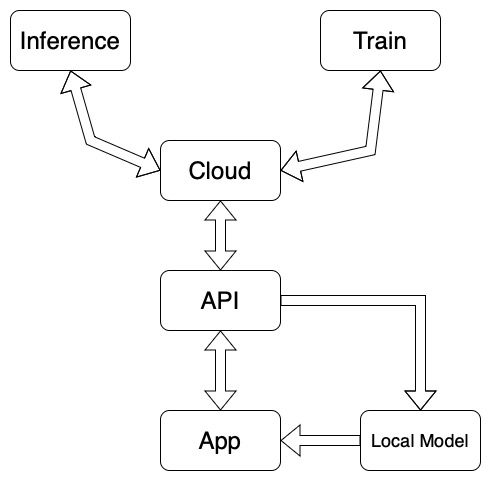
\includegraphics[width=0.4\textwidth]{Deployment}
    \caption{Deployment architecture of the system}\label{fig:deployment}
\end{figure}

Our deployment environment (Figure \ref{fig:deployment}) is in the cloud, using API access a mobile/computer app can interact with the system.
A basic model will be downloaded into the local device as well to make the communication with reduced latency.
When a user provides some basic voice command, the local model will be sufficient to reply or interact with that.
But when a complex or unknown reply is required, then it will communicate with the cloud version of the model.
The models are self-improvable, for example, it will learn to understand a specific user in a better way by user's feedback and Reinforcement Learning (RL).
Also, the local model is trained with the most commonly used commands, so that it can respond quickly for the most common words for a specific user.

The implemented Virtual Personal Assistant combines state-of-the-art technologies for speech recognition (Whisper), chatbot functionality (BanglaBERT), and Bangla text-to-speech capability.
The system effectively comprehends user speech input in the Bengali language and demonstrates the ability to accurately extract relevant answers from provided contexts using the BanglaBERT model.
This extracted information is then vocalized in Bengali through text-to-speech synthesis.

The system's performance showcases its proficiency in understanding spoken Bengali input and subsequently utilizing BanglaBERT to locate and articulate correct responses.
Although the system has not been extensively customized or fine-tuned to cater to specific user demands, the successful implementation serves as a proof-of-concept that customization is possible.
This adaptability suggests potential for tailoring the system to fulfill a wide array of user requirements.

As evidence of functionality, a provided screenshot\ref{fig:result} displays a dialogue interaction, wherein the user speaks in Bengali and the system responds appropriately.
This interaction underscores the system's real-time capabilities in processing user input, deciphering context, and generating coherent spoken Bengali output.

In summary, the Virtual Personal Assistant effectively integrates prevalent technologies to comprehend and respond to Bengali speech inputs, demonstrating its potential for customization to meet diverse user needs.

\begin{figure}
    \centering
    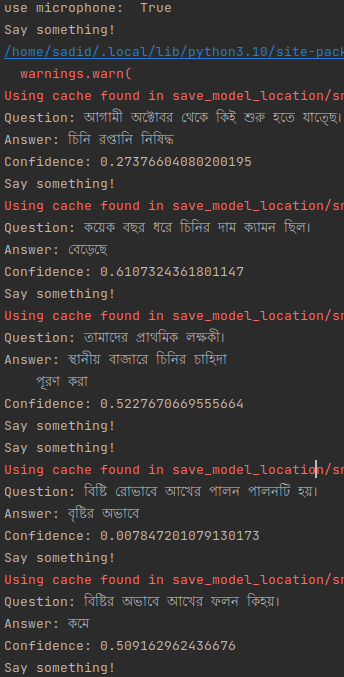
\includegraphics[width=0.4\textwidth]{result}
    \caption{Screenshot of program output}\label{fig:result}
\end{figure}



\begin{thebibliography}{00}
    \bibitem{adheetee} Syed Mohidul Islam, Most Fowziya Akther Houya, Syed Mynul Islam, Salekul Islam and Nahid Hossain, Adheetee: A Comprehensive Bangla Virtual Assistant, 2019.
    \bibitem{speech-recog-bengali} S.M. Saiful Islam Badhon, Md. Habibur Rahaman, Farea Rehnuma Rupon, State of art Research in Bengali Speech Recognition, 2020.
    \bibitem{assistant-facedetection} Dipankar Gupta, Emam Hossain, Mohammad Shahadat Hossain, Karl Andersson and Sazzad Hossain, A Digital Personal Assistant using Bangla Voice Command Recognition and Face Detection, 2019.
    \bibitem{siri-experience} Jerome R. Bellegarda, ``Large–Scale Personal Assistant Technology Deployment: the Siri Experience, 2013.
    \bibitem{rl-chatbot} Elena Ricciardelli, Debmalya Biswas, Self-improving Chatbots based on Reinforcement Learning, 2019.
    \bibitem{chatbot} Shafquat Hussain, Omid Ameri Sianaki, Nedal Ababneh, A Survey on Conversational Agents/Chatbots Classification and Design Techniques, 2019.
    \bibitem{text-to-speech} Dosik Moon, Web-Based Text-to-Speech Technologies in Foreign Language Learning: Opportunities and Challenges, 2012.
    \bibitem{doly} Md. Kowsher, Farhana Sharmin Tithi, M Ashraful Alam, Mohammad Nurul Huda, Mir Md Moheuddin, Md. Golam Rosul, Doly: Bengali Chatbot for Bengali Education, 2019.
    \bibitem{siri} AppleSiri, http://www.apple.com/ios/siri/, 011.
    \bibitem{google-mobile} Google Mobile, http://www.google.com/mobile/voice- actions, 2008.
    \bibitem{google-now} Google Now, http://www.google.com/landing/now, 2012.
    \bibitem{microsoft-tellme} Microsoft Tellme, http://www.microsoft.com/en-us/ Tellme/consumers/default.aspx, 2008.
    \bibitem{nuance-dragon} Nuance Dragon Go!, http://www.nuance.com/products/dragon-go-in-action/index.htm, 2011.
    \bibitem{nuance-nina} Nuance Nina, http://www.nuance.com/for-business/by- solution/customer-service-solutions/solutions-services/ mobile-customer-service/nina/index.htm, 2012.
    \bibitem{speaktoit} Speaktoit Assistant, http://www.speaktoit.com/index.htm, 2012.
    \bibitem{mostspoken} Chad Emery, "The 33 Most Spoken Languages in the World" Langoly https://www.asme.org/engineering-topics/articles/renewable-energy/catching-the-sun (accessed July 14, 2023).
    \bibitem{disabled-stats} Moyukh Mahtab, Faria Selim, "UNICEF concerned that more than half of children with disabilities in Bangladesh do not go to school" unicef Bangladesh https://www.unicef.org/bangladesh/en/press-releases/unicef-concerned-more-half-children-disabilities-bangladesh-do-not-go-school (accessed July 14, 2023).
    \bibitem{litaracy-bangladesh} Mir Mohammad Jasim, "Bangladesh’s slow march towards 100\% literacy" The Business Standard https://www.tbsnews.net/bangladesh/education/bangladeshs-slow-march-towards-100-literacy-492058 (accessed July 14, 2023).
    \bibitem{verbal-disabled-stats} Govt\. Bangladesh, "Report on National Survey on Persons with Disabilities (NSPD) 2021 (December 2022) [EN/BN]" reliefweb https://reliefweb.int/report/bangladesh/report-national-survey-persons-disabilities-nspd-2021-december-2022-enbn (accessed July 14, 2023).
    \bibitem{english-speaker-bangladesh} Pinon, Robert; Haydon, Jon (December 2010), The Benefits of the English Language for Individuals and Societies: Quantitative Indicators from Cameroon, Nigeria, Rwanda, Bangladesh and Pakistan, Euromonitor International Ltd
\end{thebibliography}

\end{document}
